
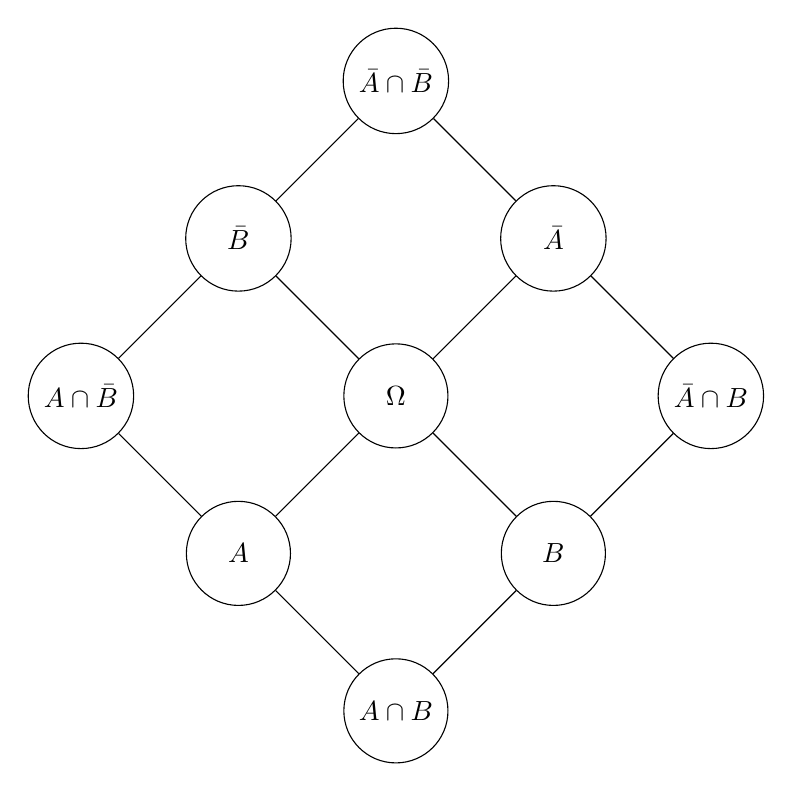
\begin{tikzpicture}[every node/.style={draw,circle,text width=1cm,align=center}]
  %\draw[help lines] (-3,-3) grid (3,3);


  \draw ( 0, 0) node[](O) {$\Omega$};

  \draw (-2,-2) node[](A)     {$A$};
  \draw ( 2,-2) node[](B)     {$B$};
  \draw ( 2, 2) node[](bA)    {$\bar{A}$};
  \draw (-2, 2) node[](bB)    {$\bar{B}$};

  \draw ( 0,-4) node[](AnB)     {$A\cap B$};
  \draw (-4, 0) node[](AnbB)     {$A\cap \bar{B}$};
  \draw ( 4, 0) node[](bAnB)     {$\bar{A}\cap B$};
  \draw ( 0, 4) node[](bAnbB)     {$\bar{A}\cap \bar{B}$};

  \path[draw] (O) -- (A) ;
  \path[draw] (O) -- (B) ;
  \path[draw] (O) -- (bA) ;
  \path[draw] (O) -- (bB) ;

  \path[draw] (A) -- (AnB);
  \path[draw] (A) -- (AnbB);

  \path[draw] (bA) -- (bAnB);
  \path[draw] (bA) -- (bAnbB);

  \path[draw] (B) -- (AnB);
  \path[draw] (B) -- (bAnB);

  \path[draw] (bB) -- (AnbB);
  \path[draw] (bB) -- (bAnbB);

\end{tikzpicture}

